\chapter{PHÂN TÍCH YÊU CẦU HỆ THỐNG}

\section{Giới thiệu chương}

Chương này trình bày quá trình khảo sát, phân tích và đặc tả yêu cầu của hệ thống \textbf{AITasker – AI Marketplace Platform for AI Automation Services}. Đây là giai đoạn quan trọng trong quá trình phát triển phần mềm, giúp xác định rõ bài toán cần giải quyết, phạm vi của hệ thống, các yêu cầu nghiệp vụ cũng như các yêu cầu kỹ thuật làm cơ sở cho việc thiết kế và triển khai ở các chương tiếp theo.
Trước hết, chương tiến hành khảo sát thực trạng của thị trường dịch vụ AI, phân tích những khó khăn mà doanh nghiệp và các chuyên gia AI đang gặp phải trong quá trình tìm kiếm, kết nối và hợp tác triển khai các dự án AI. Trên cơ sở đó, hệ thống được đề xuất nhằm giải quyết các vấn đề còn tồn tại, đồng thời đáp ứng nhu cầu ngày càng tăng về ứng dụng AI trong doanh nghiệp.
Tiếp theo, chương xây dựng tài liệu đặc tả yêu cầu phần mềm (Software Requirement Specification -- SRS), bao gồm việc xác định các tác nhân tham gia hệ thống, mô tả chức năng của từng nhóm người dùng và phân tích các yêu cầu chức năng, yêu cầu phi chức năng cũng như các ràng buộc cần đáp ứng. Những nội dung này là nền tảng để đảm bảo hệ thống được xây dựng đúng với mục tiêu và đáp ứng các yêu cầu của người sử dụng.
Bên cạnh đó, chương sử dụng ngôn ngữ mô hình hóa UML để mô tả trực quan các nghiệp vụ và quy trình xử lý của hệ thống thông qua các biểu đồ như Use Case Diagram, Activity Diagram, Sequence Diagram và Class Diagram. Đồng thời, mô hình dữ liệu được xây dựng bằng Entity Relationship Diagram (ERD) nhằm xác định các thực thể, thuộc tính và mối quan hệ giữa chúng, phục vụ cho việc thiết kế cơ sở dữ liệu của hệ thống.
Thông qua quá trình phân tích và mô hình hóa, các chức năng cốt lõi của nền tảng như quản lý người dùng, quản lý dự án AI, quản lý đề xuất (Proposal), trao đổi giữa doanh nghiệp và chuyên gia, quản lý tiến độ dự án, đánh giá sau khi hoàn thành dự án và quản trị hệ thống được xác định một cách đầy đủ và rõ ràng. Đồng thời, chương cũng làm rõ luồng tương tác giữa các thành phần của hệ thống, góp phần đảm bảo tính nhất quán trong quá trình thiết kế và phát triển.
Kết quả của chương là bộ tài liệu phân tích và đặc tả yêu cầu hoàn chỉnh, đóng vai trò làm nền tảng cho việc thiết kế kiến trúc hệ thống, thiết kế cơ sở dữ liệu, xây dựng các thành phần phần mềm và triển khai nền tảng \textbf{AITasker} trong các chương tiếp theo.
\section{Mô tả bài toán}

\subsection{Bối cảnh}

Trong bối cảnh cuộc Cách mạng công nghiệp lần thứ tư (Industry 4.0) và quá trình chuyển đổi số đang diễn ra mạnh mẽ trên phạm vi toàn cầu, trí tuệ nhân tạo (Artificial Intelligence -- AI) đã trở thành một trong những công nghệ nền tảng thúc đẩy đổi mới sáng tạo và nâng cao năng lực cạnh tranh của doanh nghiệp. AI được ứng dụng rộng rãi trong nhiều lĩnh vực như chăm sóc khách hàng, thương mại điện tử, tài chính, y tế, giáo dục, sản xuất, logistics và quản trị doanh nghiệp nhằm tự động hóa quy trình, phân tích dữ liệu, tối ưu hoạt động và hỗ trợ ra quyết định.
Trong những năm gần đây, sự phát triển vượt bậc của các công nghệ như Machine Learning, Deep Learning, Natural Language Processing (NLP), Computer Vision, Generative AI và Large Language Models (LLMs) đã mở ra nhiều cơ hội mới trong việc xây dựng các giải pháp AI có tính ứng dụng cao. Các mô hình AI hiện đại không chỉ giúp doanh nghiệp xử lý dữ liệu với quy mô lớn mà còn có khả năng tạo nội dung, phân tích tài liệu, xây dựng chatbot thông minh, trợ lý ảo và tự động hóa nhiều quy trình nghiệp vụ. Nhờ đó, việc ứng dụng AI ngày càng trở nên phổ biến và có chi phí triển khai phù hợp hơn đối với cả doanh nghiệp lớn lẫn doanh nghiệp vừa và nhỏ.
Cùng với sự phát triển của công nghệ, nhu cầu triển khai các dự án AI trong doanh nghiệp cũng gia tăng nhanh chóng. Nhiều tổ chức mong muốn ứng dụng AI để nâng cao chất lượng dịch vụ, tối ưu quy trình vận hành, giảm chi phí nhân sự và tạo ra các sản phẩm, dịch vụ thông minh. Tuy nhiên, quá trình triển khai các giải pháp AI thường đòi hỏi nguồn nhân lực có trình độ chuyên môn cao về khoa học dữ liệu, phát triển phần mềm, điện toán đám mây, xử lý dữ liệu và các thuật toán học máy. Đây là thách thức lớn đối với nhiều doanh nghiệp khi nguồn nhân lực AI chất lượng cao còn hạn chế và chi phí xây dựng đội ngũ nội bộ tương đối lớn.
Bên cạnh đó, các chuyên gia AI, freelancer và các công ty cung cấp dịch vụ AI cũng gặp không ít khó khăn trong việc tiếp cận khách hàng có nhu cầu thực tế. Phần lớn việc tìm kiếm dự án hiện nay vẫn thông qua các nền tảng freelancer tổng quát hoặc các kênh mạng xã hội, vốn chưa được thiết kế chuyên biệt cho lĩnh vực AI. Điều này khiến quá trình kết nối giữa doanh nghiệp và chuyên gia thiếu tính minh bạch, khó đánh giá năng lực chuyên môn, đồng thời chưa hỗ trợ đầy đủ các nghiệp vụ như quản lý dự án, báo giá, theo dõi tiến độ hay đánh giá chất lượng sau khi hoàn thành dự án.
Xuất phát từ thực trạng trên, việc xây dựng một nền tảng Marketplace chuyên biệt dành cho các dịch vụ AI là nhu cầu cần thiết. Một hệ thống như vậy sẽ đóng vai trò là cầu nối giữa doanh nghiệp và các chuyên gia AI, hỗ trợ toàn bộ quá trình hợp tác từ đăng tải yêu cầu, tìm kiếm chuyên gia, gửi đề xuất (Proposal), trao đổi thông tin, quản lý tiến độ, thanh toán đến đánh giá sau dự án. Không chỉ góp phần nâng cao hiệu quả triển khai các dự án AI, nền tảng còn thúc đẩy quá trình chuyển đổi số của doanh nghiệp và tạo môi trường phát triển bền vững cho cộng đồng chuyên gia AI.
\subsection{Thực trạng}

Hiện nay, cùng với sự phát triển mạnh mẽ của trí tuệ nhân tạo, nhu cầu triển khai các giải pháp AI trong doanh nghiệp ngày càng gia tăng. Tuy nhiên, thị trường cung cấp dịch vụ AI vẫn chưa có nhiều nền tảng chuyên biệt hỗ trợ kết nối hiệu quả giữa doanh nghiệp và các chuyên gia AI. Phần lớn doanh nghiệp hiện nay vẫn tìm kiếm đối tác thông qua các nền tảng tuyển dụng, marketplace freelancer hoặc các mạng xã hội nghề nghiệp. Mặc dù những kênh này sở hữu cộng đồng người dùng lớn, chúng chủ yếu phục vụ nhiều lĩnh vực khác nhau và chưa được thiết kế để đáp ứng các đặc thù của các dự án AI.
Đối với doanh nghiệp, việc tìm kiếm một chuyên gia hoặc đơn vị cung cấp dịch vụ AI phù hợp thường gặp nhiều khó khăn. Do đặc thù của lĩnh vực AI đòi hỏi kiến thức chuyên môn sâu về Machine Learning, Deep Learning, xử lý dữ liệu, phát triển mô hình và triển khai hệ thống, việc đánh giá năng lực của ứng viên thông qua hồ sơ hoặc thông tin giới thiệu là chưa đủ. Nhiều doanh nghiệp thiếu tiêu chí và công cụ để đánh giá chính xác kinh nghiệm thực tế, khả năng triển khai dự án cũng như chất lượng sản phẩm của các chuyên gia.
Ở chiều ngược lại, các chuyên gia AI, freelancer và các nhóm phát triển giải pháp AI cũng gặp khó khăn trong việc tiếp cận các doanh nghiệp có nhu cầu thực sự. Họ thường phải phụ thuộc vào các nền tảng freelancer tổng quát hoặc tự xây dựng thương hiệu cá nhân thông qua các kênh truyền thông. Điều này làm giảm khả năng tiếp cận các dự án phù hợp, đồng thời khiến quá trình xây dựng uy tín và mở rộng thị trường trở nên khó khăn hơn.
Bên cạnh đó, quá trình triển khai một dự án AI thường bao gồm nhiều giai đoạn như tiếp nhận yêu cầu, phân tích bài toán, gửi đề xuất (Proposal), thương lượng, quản lý tiến độ, nghiệm thu, thanh toán và đánh giá sau dự án. Trong thực tế, các hoạt động này thường được thực hiện thông qua nhiều công cụ riêng biệt như email, ứng dụng nhắn tin, lưu trữ đám mây hoặc các phần mềm quản lý công việc, dẫn đến dữ liệu bị phân tán, khó kiểm soát và thiếu tính đồng bộ trong quá trình hợp tác.
Một số hạn chế nổi bật của các nền tảng hiện nay có thể được tổng hợp như sau:

\begin{itemize}
    \item Khó đánh giá chính xác năng lực chuyên môn, kinh nghiệm triển khai và chất lượng công việc của các chuyên gia AI.
    \item Quá trình tìm kiếm, sàng lọc và lựa chọn chuyên gia phù hợp còn mất nhiều thời gian, chi phí và phụ thuộc nhiều vào đánh giá thủ công.
    \item Thiếu nền tảng chuyên biệt hỗ trợ doanh nghiệp và chuyên gia AI trao đổi yêu cầu kỹ thuật, gửi báo giá (Proposal), thương lượng và quản lý hợp đồng.
    \item Chưa hỗ trợ quản lý xuyên suốt vòng đời dự án AI, bao gồm theo dõi tiến độ, quản lý các mốc công việc (Milestone), lưu trữ tài liệu, lịch sử trao đổi và quá trình nghiệm thu.
    \item Hệ thống đánh giá, xếp hạng và phản hồi sau dự án còn hạn chế, gây khó khăn trong việc xây dựng uy tín và mức độ tin cậy giữa các bên.
    \item Chưa khai thác hiệu quả các công nghệ AI để gợi ý chuyên gia phù hợp với yêu cầu của doanh nghiệp hoặc đề xuất các dự án phù hợp với hồ sơ năng lực, kỹ năng và kinh nghiệm của chuyên gia.
    \item Khả năng tích hợp các dịch vụ hỗ trợ như thanh toán trực tuyến, thông báo theo thời gian thực, quản lý tài liệu và báo cáo tiến độ còn chưa đồng bộ, làm giảm hiệu quả phối hợp trong quá trình triển khai dự án.
\end{itemize}

Ở chiều ngược lại, các chuyên gia AI, freelancer và các nhóm phát triển giải pháp AI cũng gặp nhiều khó khăn trong việc tiếp cận khách hàng có nhu cầu thực sự. Nhiều chuyên gia phải tìm kiếm dự án thông qua các kênh trung gian hoặc mạng xã hội, dẫn đến khả năng tiếp cận khách hàng còn hạn chế, khó xây dựng uy tín cá nhân và mất nhiều thời gian trong quá trình tìm kiếm cơ hội hợp tác.
Từ những hạn chế trên, có thể thấy việc xây dựng một nền tảng chuyên biệt dành cho các dịch vụ AI là cần thiết. Nền tảng sẽ giúp kết nối doanh nghiệp với chuyên gia AI một cách hiệu quả, đồng thời hỗ trợ quản lý toàn bộ quy trình hợp tác từ đăng dự án, gửi báo giá, trao đổi, theo dõi tiến độ đến đánh giá sau khi hoàn thành dự án.
\subsection{Giải pháp đề xuất}

Đề tài xây dựng hệ thống AIConnect nhằm kết nối doanh nghiệp với các chuyên gia AI. Hệ thống hỗ trợ doanh nghiệp đăng tải dự án, tìm kiếm chuyên gia, ký kết hợp đồng, quản lý tiến độ và thanh toán trực tuyến.

Đối với chuyên gia AI, hệ thống cho phép tạo hồ sơ năng lực, tìm kiếm dự án, gửi đề xuất hợp tác và trao đổi trực tiếp với doanh nghiệp. Ngoài ra, hệ thống còn tích hợp chức năng AI Matching nhằm đề xuất chuyên gia phù hợp dựa trên kỹ năng, kinh nghiệm và lịch sử dự án.

\section{Đặc tả yêu cầu phần mềm (SRS)}

\subsection{Mục tiêu hệ thống}

AIConnect được xây dựng nhằm tạo ra nền tảng trung gian giúp doanh nghiệp và chuyên gia AI kết nối với nhau một cách nhanh chóng, minh bạch và hiệu quả. Hệ thống hỗ trợ toàn bộ quy trình từ đăng dự án, tìm kiếm chuyên gia, gửi đề xuất, ký hợp đồng, quản lý tiến độ, thanh toán đến đánh giá sau khi hoàn thành dự án.

\subsection{Đối tượng sử dụng}

Hệ thống gồm ba nhóm người dùng chính:
\begin{itemize}
    \item \textbf{Doanh nghiệp (Enterprise):} Đơn vị có nhu cầu giải quyết các bài toán AI.
    \item \textbf{Chuyên gia AI (Expert):} Cá nhân hoặc nhóm có năng lực triển khai giải pháp AI.
    \item \textbf{Quản trị viên (Admin):} Đơn vị vận hành và kiểm duyệt nền tảng.
\end{itemize}

\subsection{Yêu cầu chức năng}

\begin{table}[H]
\centering
\caption{Danh sách yêu cầu chức năng hệ thống}
\label{tab:functional_requirements}
\renewcommand{\arraystretch}{1.2}
\begin{tabular}{|c|p{8cm}|p{4cm}|}
\hline
\textbf{Mã} & \textbf{Mô tả yêu cầu} & \textbf{Tác nhân}\\
\hline
FR01 & Đăng ký tài khoản & Tất cả tác nhân\\
\hline
FR02 & Đăng nhập hệ thống & Tất cả tác nhân\\
\hline
FR03 & Quản lý hồ sơ cá nhân & Tất cả tác nhân\\
\hline
FR04 & Đăng dự án AI & Doanh nghiệp\\
\hline
FR05 & Tìm kiếm chuyên gia & Doanh nghiệp\\
\hline
FR06 & AI Matching chuyên gia & Doanh nghiệp\\
\hline
FR07 & Tạo hồ sơ chuyên gia & Chuyên gia\\
\hline
FR08 & Gửi đề xuất dự án & Chuyên gia\\
\hline
FR09 & Thuê chuyên gia & Doanh nghiệp\\
\hline
FR10 & Quản lý hợp đồng & Doanh nghiệp, Chuyên gia\\
\hline
FR11 & Quản lý tiến độ & Doanh nghiệp, Chuyên gia\\
\hline
FR12 & Chat trực tuyến & Doanh nghiệp, Chuyên gia\\
\hline
FR13 & Thanh toán trực tuyến & Doanh nghiệp\\
\hline
FR14 & Đánh giá dự án & Doanh nghiệp, Chuyên gia\\
\hline
FR15 & Quản lý người dùng & Admin\\
\hline
FR16 & Quản lý nội dung và kiểm duyệt & Admin\\
\hline
FR17 & Thống kê hệ thống & Admin\\
\hline
\end{tabular}
\end{table}

\subsection{Yêu cầu phi chức năng}

\begin{table}[H]
\centering
\caption{Danh sách yêu cầu phi chức năng}
\label{tab:non_functional_requirements}
\renewcommand{\arraystretch}{1.2}
\begin{tabular}{|c|p{12cm}|}
\hline
\textbf{Mã} & \textbf{Mô tả chi tiết kỹ thuật}\\
\hline
NFR01 & Thời gian phản hồi hệ thống nhỏ hơn 2 giây với các tác vụ thông thường.\\
\hline
NFR02 & Hỗ trợ tối thiểu 500 người dùng truy cập đồng thời tại một thời điểm.\\
\hline
NFR03 & Toàn bộ hệ thống giao tiếp qua giao thức bảo mật HTTPS.\\
\hline
NFR04 & Cơ chế xác thực phân quyền sử dụng JWT (JSON Web Token).\\
\hline
NFR05 & Mật khẩu người dùng được mã hóa một chiều bằng thuật toán BCrypt.\\
\hline
NFR06 & Hệ thống hoạt động liên tục với độ sẵn sàng cao 24/7.\\
\hline
NFR07 & Kiến trúc có khả năng mở rộng theo chiều ngang (Horizontal Scaling).\\
\hline
NFR08 & Hỗ trợ triển khai linh hoạt trên các nền tảng điện toán đám mây (Cloud).\\
\hline
NFR09 & Giao diện thích ứng (Responsive UI), thân thiện với người dùng.\\
\hline
NFR10 & Độ sẵn sàng của dịch vụ cốt lõi đạt tối thiểu 99.5\%.\\
\hline
\end{tabular}
\end{table}

\section{Xác định tác nhân hệ thống}

\subsection{Doanh nghiệp (Enterprise)}
Tác nhân đại diện cho các tổ chức, công ty có nhu cầu tìm kiếm nguồn lực công nghệ bên ngoài:
\begin{itemize}
    \item Đăng ký, đăng nhập và cập nhật hồ sơ pháp lý doanh nghiệp.
    \item Đăng tải thông tin, mô tả bài toán và ngân sách dự án AI.
    \item Sàng lọc, tìm kiếm và nhận đề xuất từ các chuyên gia.
    \item Phê duyệt đề xuất, ký kết hợp đồng điện tử và quản lý tiến độ.
    \item Giải ngân, thanh toán cột mốc và thực hiện đánh giá chuyên gia.
\end{itemize}

\subsection{Chuyên gia AI (Expert)}

Tác nhân đại diện cho các kỹ sư AI, nhà khoa học dữ liệu (Data Scientist), kỹ sư Machine Learning, kỹ sư MLOps, chuyên gia tự động hóa AI, freelancer hoặc các nhóm phát triển giải pháp AI có nhu cầu tìm kiếm cơ hội hợp tác với doanh nghiệp. Đây là nhóm người dùng trực tiếp cung cấp các dịch vụ AI trên nền tảng.

\begin{itemize}
    \item Đăng ký, đăng nhập và quản lý thông tin tài khoản cá nhân.
    \item Xây dựng hồ sơ năng lực (Portfolio), cập nhật thông tin cá nhân, kỹ năng, chứng chỉ, kinh nghiệm làm việc, dự án đã thực hiện và các lĩnh vực chuyên môn.
    \item Thiết lập danh mục dịch vụ AI cung cấp và mức giá tham khảo.
    \item Tìm kiếm, lọc và theo dõi các dự án AI phù hợp với kỹ năng, kinh nghiệm và lĩnh vực chuyên môn.
    \item Gửi Proposal (đề xuất thực hiện dự án), báo giá, thời gian triển khai và kế hoạch thực hiện cho doanh nghiệp.
    \item Trao đổi trực tiếp với doanh nghiệp thông qua hệ thống nhắn tin để làm rõ yêu cầu, thương lượng ngân sách và phạm vi công việc.
    \item Tham gia triển khai dự án sau khi được doanh nghiệp lựa chọn.
    \item Cập nhật tiến độ thực hiện, quản lý các mốc công việc (Milestones), tải lên tài liệu, sản phẩm và báo cáo kết quả trong quá trình triển khai.
    \item Theo dõi trạng thái dự án, lịch sử hợp tác, các khoản thanh toán và doanh thu từ các dự án đã hoàn thành.
    \item Nhận thanh toán sau khi dự án hoặc từng mốc công việc được doanh nghiệp nghiệm thu.
    \item Đánh giá và phản hồi doanh nghiệp sau khi kết thúc dự án nhằm xây dựng môi trường hợp tác minh bạch và nâng cao chất lượng dịch vụ.
\end{itemize}

\subsection{Quản trị viên (Admin)}

Quản trị viên là tác nhân chịu trách nhiệm quản lý, vận hành và giám sát toàn bộ nền tảng nhằm đảm bảo hệ thống hoạt động ổn định, an toàn và minh bạch. Admin có quyền truy cập cao nhất và thực hiện các nghiệp vụ quản trị liên quan đến người dùng, dự án và hệ thống.

\begin{itemize}
    \item Quản lý toàn bộ tài khoản người dùng, bao gồm doanh nghiệp, chuyên gia AI và các tài khoản quản trị.
    \item Phê duyệt, khóa, mở khóa hoặc phân quyền tài khoản khi cần thiết.
    \item Kiểm duyệt các bài đăng dự án, hồ sơ chuyên gia và nội dung trên nền tảng nhằm đảm bảo tuân thủ các quy định và chính sách của hệ thống.
    \item Giám sát quá trình hợp tác giữa doanh nghiệp và chuyên gia, hỗ trợ xử lý các khiếu nại, tranh chấp hoặc vi phạm trong quá trình thực hiện dự án.
    \item Quản lý các giao dịch tài chính, theo dõi thanh toán, giải ngân và kiểm tra các giao dịch bất thường.
    \item Quản lý danh mục kỹ năng, lĩnh vực AI, danh mục dịch vụ và các dữ liệu dùng chung của hệ thống.
    \item Theo dõi tình trạng hoạt động của hệ thống, giám sát nhật ký (Log), hiệu năng và các cảnh báo bảo mật.
    \item Thống kê, tổng hợp và phân tích dữ liệu hoạt động của nền tảng thông qua các báo cáo về số lượng người dùng, dự án, doanh thu, giao dịch và các chỉ số tăng trưởng.
    \item Quản lý cấu hình hệ thống, gửi thông báo đến người dùng và hỗ trợ bảo trì, nâng cấp hệ thống khi cần thiết.
\end{itemize}

\section{Danh sách Use Case}

Mô hình Use Case tổng thể được bóc tách chi tiết thông qua các hành vi đặc trưng của từng tác nhân được liệt kê chi tiết trong Bảng \ref{tab:usecase}.

\begin{table}[H]
\centering
\caption{Danh sách Use Case của hệ thống AIConnect}
\label{tab:usecase}
\renewcommand{\arraystretch}{1.2}
\begin{tabular}{|c|p{8cm}|p{4cm}|}
\hline
\textbf{Mã} & \textbf{Tên Use Case} & \textbf{Tác nhân}\\
\hline
UC01 & Đăng ký tài khoản & Tất cả tác nhân\\
\hline
UC02 & Đăng nhập hệ thống & Tất cả tác nhân\\
\hline
UC03 & Quản lý hồ sơ cá nhân & Tất cả tác nhân\\
\hline
UC04 & Đăng dự án AI & Doanh nghiệp\\
\hline
UC05 & Tìm kiếm chuyên gia & Doanh nghiệp\\
\hline
UC06 & AI Matching chuyên gia & Doanh nghiệp\\
\hline
UC07 & Tạo hồ sơ chuyên gia & Chuyên gia\\
\hline
UC08 & Gửi đề xuất dự án & Chuyên gia\\
\hline
UC09 & Thuê chuyên gia & Doanh nghiệp\\
\hline
UC10 & Quản lý hợp đồng & Doanh nghiệp, Chuyên gia\\
\hline
UC11 & Quản lý tiến độ dự án & Doanh nghiệp, Chuyên gia\\
\hline
UC12 & Chat trực tuyến & Doanh nghiệp, Chuyên gia\\
\hline
UC13 & Thanh toán trực tuyến & Doanh nghiệp\\
\hline
UC14 & Đánh giá dự án & Doanh nghiệp, Chuyên gia\\
\hline
UC15 & Quản lý người dùng & Admin\\
\hline
UC16 & Kiểm duyệt nội dung & Admin\\
\hline
UC17 & Xem thống kê hệ thống & Admin\\
\hline
\end{tabular}
\end{table}

\section{Biểu đồ Use Case}

Biểu đồ Use Case mô tả trực quan các ranh giới chức năng chính của hệ thống và mối tương quan tương tác giữa các nhóm tác nhân với nền tảng.

\begin{figure}[H]
\centering
\includegraphics[width=0.3\textwidth]{figures/usecase.png}
\caption{Biểu đồ Use Case tổng thể hệ thống AIConnect}
\label{fig:usecase_diagram}
\end{figure}

Thông qua mô hình hóa Use Case, luồng chức năng phân hệ được phân định rõ ràng. Doanh nghiệp nắm giữ các quyền cốt lõi về mặt tài chính và điều phối công việc như đăng bài, chọn đối tác và thanh toán. Chuyên gia tập trung vào các hành vi thể hiện năng lực và phản hồi kết quả công việc. Trong khi đó, nhóm Admin vận hành độc lập ở phân hệ quản trị hệ thống.

\section{Biểu đồ Activity}

\subsection{Activity Diagram chức năng đăng nhập}
Biểu đồ hoạt động mô tả tiến trình xác thực danh tính người dùng khi truy cập vào hệ thống nền tảng.

\begin{figure}[H]
\centering
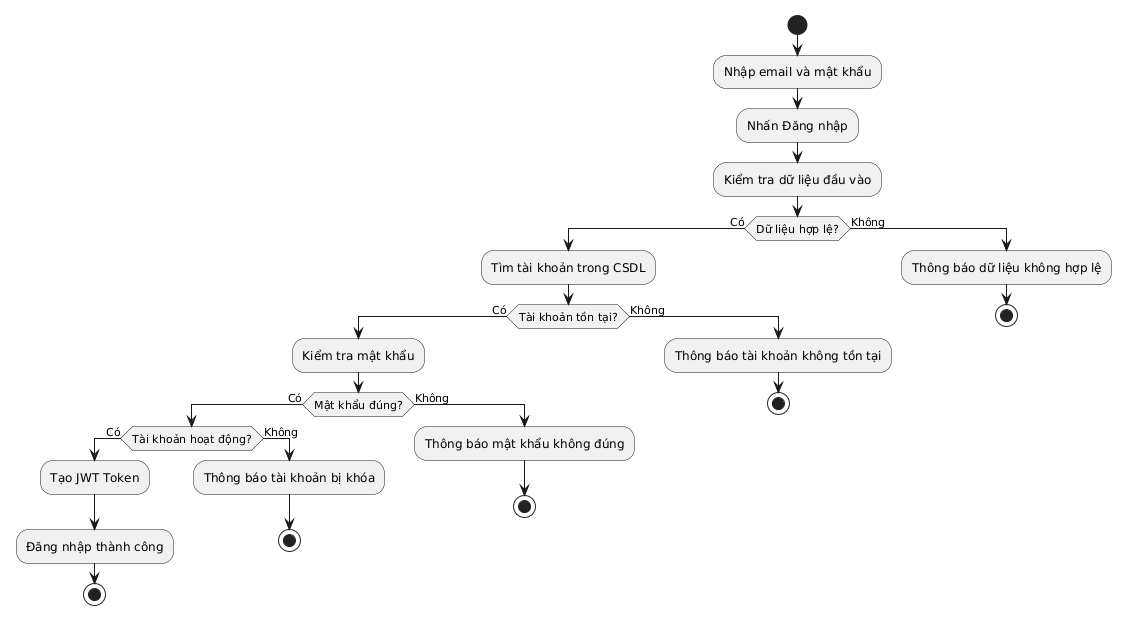
\includegraphics[width=0.7\textwidth]{figures/activity1.png}
\caption{Activity Diagram chức năng đăng nhập}
\label{fig:activity_login}
\end{figure}

Quy trình bắt đầu khi người dùng nhập thông tin định danh bao gồm Email và Mật khẩu. Hệ thống tiến hành truy vấn kiểm tra sự tồn tại của tài khoản trong cơ sở dữ liệu. Nếu tài khoản không tồn tại hoặc mật khẩu băm đối sánh (BCrypt) không trùng khớp, hệ thống sẽ trả về thông báo lỗi và yêu cầu nhập lại. Nếu thông tin hoàn toàn hợp lệ, hệ thống tiến hành cấp phát mã mã hóa JWT Token, chuyển hướng người dùng vào trang giao diện Dashboard tương ứng với vai trò của họ.

\subsection{Activity Diagram chức năng đăng tải dự án}
Biểu đồ mô tả luồng nghiệp vụ khi tác nhân Doanh nghiệp khởi tạo và công bố một bài toán công nghệ mới lên cộng đồng.

\begin{figure}[H]
\centering
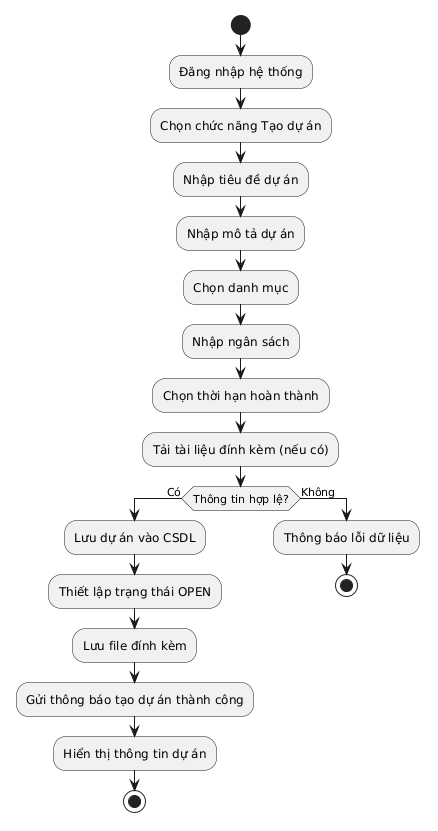
\includegraphics[width=0.45\textwidth]{figures/activity2.png}
\caption{Activity Diagram chức năng đăng tải dự án}
\label{fig:activity_create_project}
\end{figure}

Doanh nghiệp chọn tính năng đăng dự án và hoàn thiện biểu mẫu thông tin (Tiêu đề, mô tả bài toán, ngân sách, yêu cầu kỹ thuật và danh mục công nghệ). Hệ thống sẽ thực hiện kiểm tra tính hợp lệ của dữ liệu đầu vào. Tiếp theo, hệ thống rẽ nhánh kiểm tra sự tồn tại của tệp tài liệu đính kèm kèm theo. Nếu có, tệp tin sẽ được tải lên hệ thống lưu trữ và liên kết đường dẫn. Sau khi hoàn tất lưu bản ghi dự án với trạng thái \texttt{OPEN}, hệ thống kích hoạt Dịch vụ thông báo để lưu log đồng thời hiển thị thông báo thành công ra màn hình Client.

\subsection{Activity Diagram chức năng gửi đề xuất}
Biểu đồ hoạt động mô tả chi tiết quy trình nghiệp vụ và các bước kiểm tra logic khi chuyên gia AI chủ động nộp hồ sơ giải pháp cho dự án.

\begin{figure}[H]
\centering
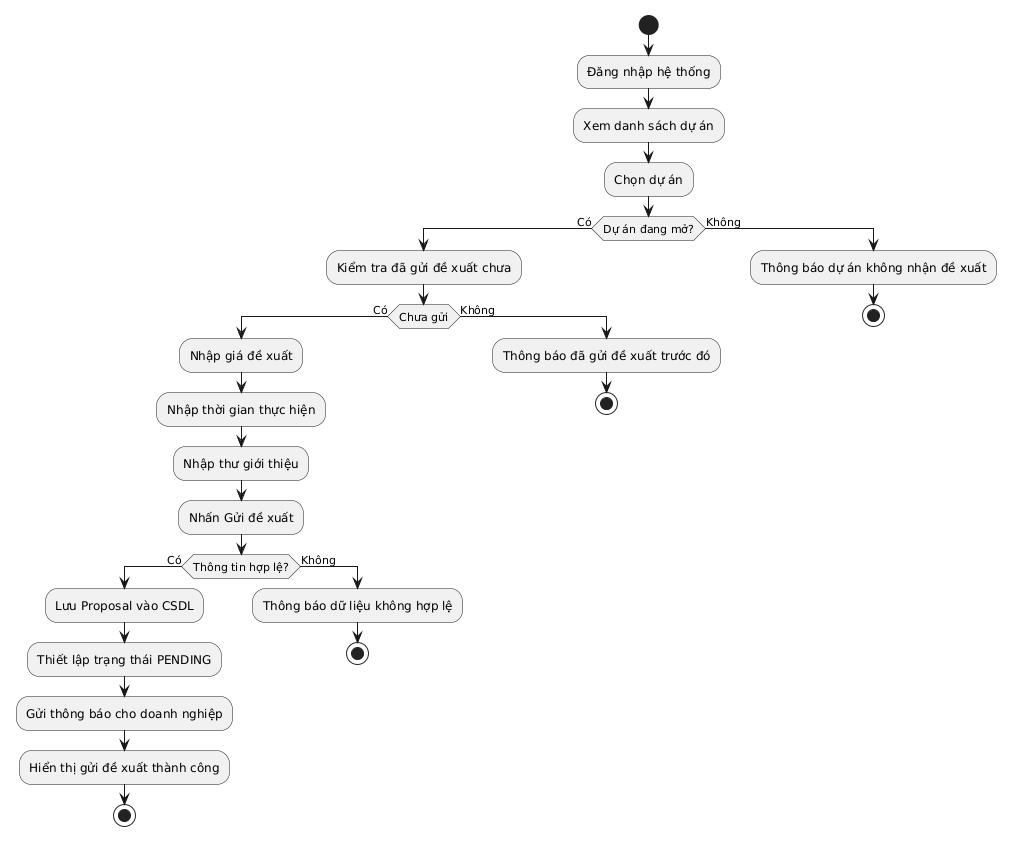
\includegraphics[width=0.7\textwidth]{figures/activity3.png}
\caption{Activity Diagram chức năng gửi đề xuất dự án}
\label{fig:activity_submit_proposal}
\end{figure}

Quy trình nghiệp vụ yêu cầu chuyên gia phải đăng nhập hợp lệ. Khi một dự án được chọn, hệ thống sẽ chạy tiến trình kiểm tra trạng thái song song: đảm bảo dự án vẫn trong thời hạn nhận hồ sơ và chuyên gia này chưa từng nộp đề xuất nào trước đó. Form nhập liệu yêu cầu đầy đủ các thông số tài chính và kỹ thuật trước khi lưu dữ liệu xuống phân hệ lưu trữ.

\subsection{Activity Diagram chức năng thuê chuyên gia}
Sơ đồ mô tả quy trình chuyển đổi trạng thái mang tính chất giao dịch khi doanh nghiệp chấp thuận một chuyên gia thực hiện dự án.

\begin{figure}[H]
\centering
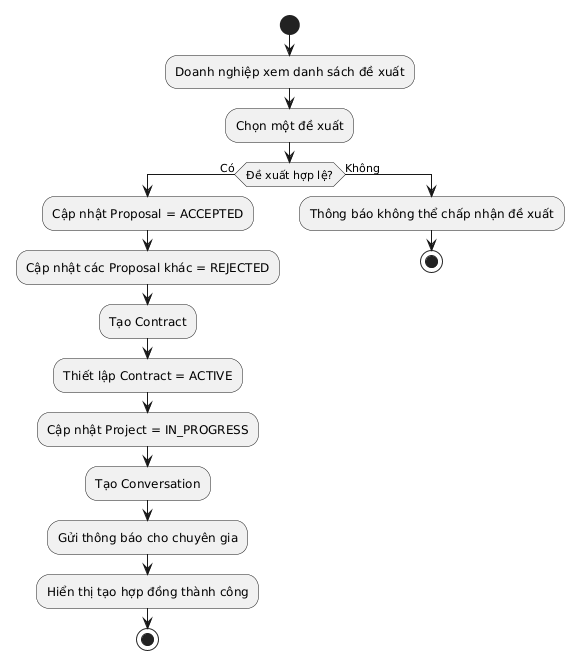
\includegraphics[width=0.7\textwidth]{figures/activity4.png}
\caption{Activity Diagram chức năng thuê chuyên gia và tạo hợp đồng}
\label{fig:activity_hire_expert}
\end{figure}

Tiến trình xử lý tự động hóa của hệ thống đảm bảo tính toàn vẹn: khi một đề xuất chuyển sang trạng thái \texttt{ACCEPTED}, toàn bộ các đề xuất ứng tuyển đồng cấp khác lập tức chuyển thành \texttt{REJECTED}. Các thực thể phụ thuộc như Hợp đồng mới và Kênh giao tiếp thời gian thực cũng đồng thời được khởi tạo trong cùng một phiên xử lý.

\subsection{Activity Diagram chức năng thanh toán}
Biểu đồ hoạt động mô tả quy trình giải ngân tài chính cho từng cột mốc công việc dựa trên việc kết nối với cổng thanh toán điện tử ngoại vi.

\begin{figure}[H]
\centering
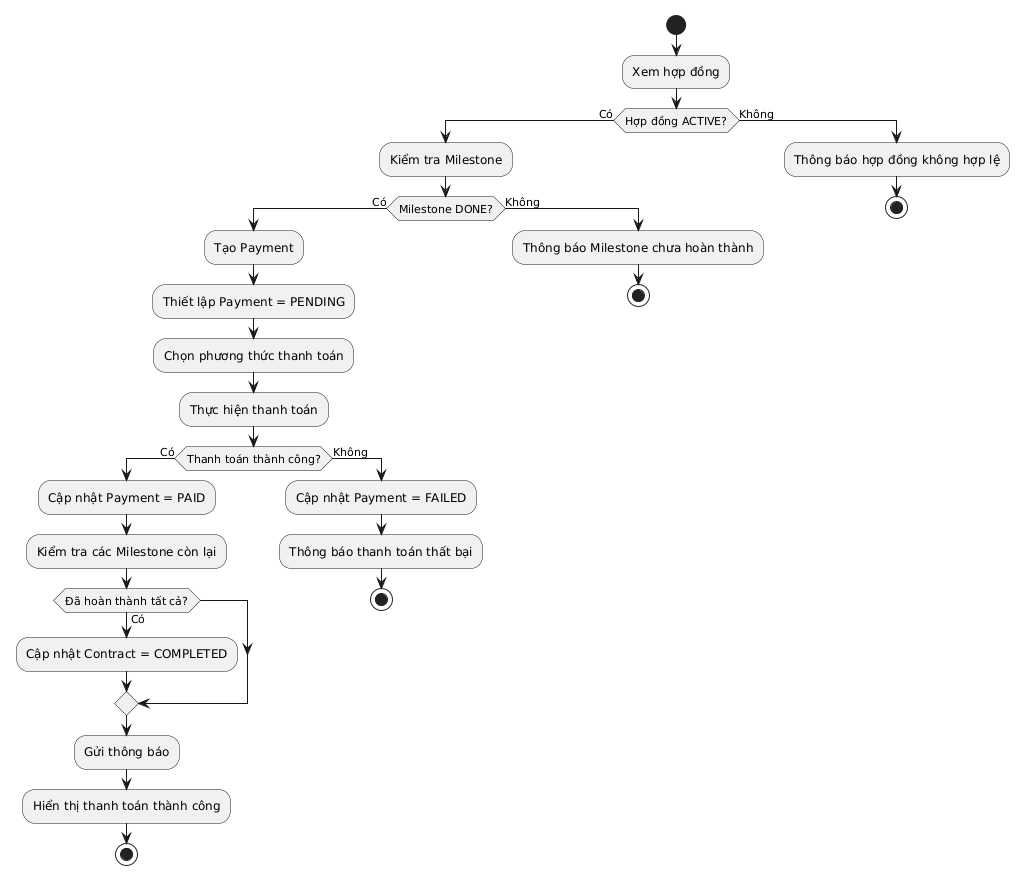
\includegraphics[width=0.7\textwidth]{figures/activity5.png}
\caption{Activity Diagram chức năng thanh toán giai đoạn}
\label{fig:activity_payment}
\end{figure}

Doanh nghiệp thực hiện kích hoạt lệnh giải ngân cho một cột mốc công việc đã được nghiệm thu kỹ thuật. Hệ thống kiểm tra điều kiện trạng thái của hợp đồng (\texttt{ACTIVE}) và trạng thái cột mốc (\texttt{DONE}). Nếu hợp lệ, một bản ghi giao dịch với trạng thái \texttt{PENDING} được thiết lập và hệ thống điều hướng người dùng sang giao diện của bên thứ ba (Cổng thanh toán). Tùy thuộc vào gói tin phản hồi trả về, hệ thống cập nhật kết quả thành \texttt{PAID} (Thành công) hoặc \texttt{FAILED} (Thất bại), ghi nhận vào nhật ký hệ thống và phát thông báo đến cả hai bên tác nhân.

\subsection{Activity Diagram chức năng đánh giá dự án}
Luồng hoạt động đóng vai trò chốt chặn cuối cùng nhằm cập nhật chỉ số uy tín của các bên sau khi hợp đồng kết thúc.

\begin{figure}[H]
\centering
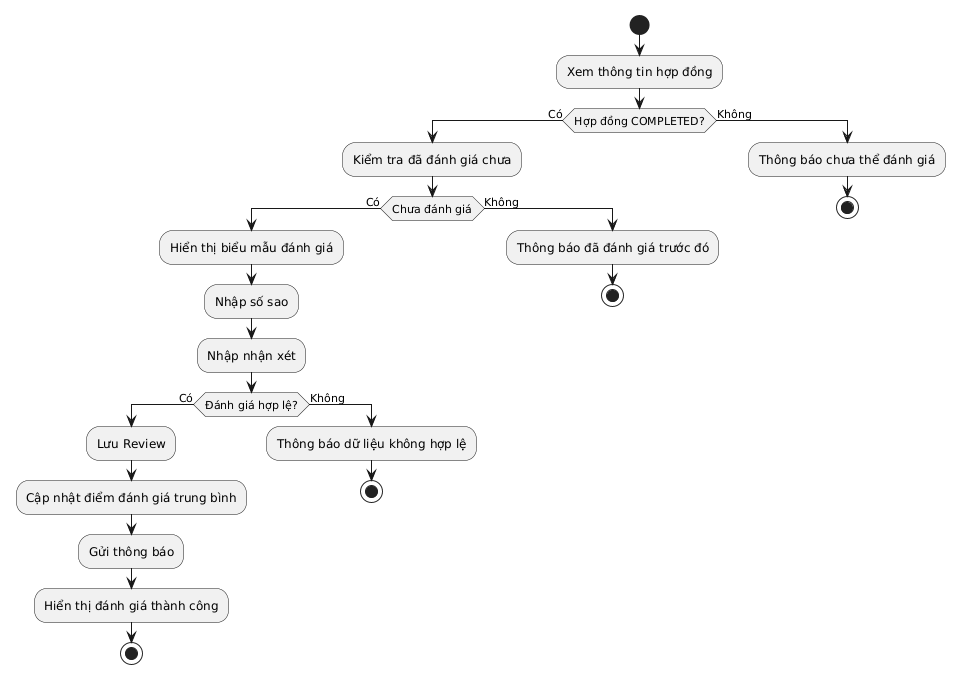
\includegraphics[width=0.7\textwidth]{figures/activity6.png}
\caption{Activity Diagram chức năng đánh giá kết quả dự án}
\label{fig:activity_review_project}
\end{figure}

Hệ thống chỉ kích hoạt quyền đánh giá khi kiểm tra bản ghi hợp đồng đã chuyển hẳn sang trạng thái \texttt{COMPLETED}. Điểm số sao (\texttt{rating}) sau khi được biểu mẫu thu thập sẽ được đưa vào hàm thuật toán tính toán lại điểm trung bình tích lũy trước khi cập nhật trực tiếp vào hồ sơ tổng của người dùng.

\section{Biểu đồ Sequence}

\subsection{Sequence Diagram chức năng đăng nhập}
Mô tả trình tự trao đổi thông điệp xác thực an toàn giữa Client và Server sử dụng cơ chế chữ ký điện tử JWT.

\begin{figure}[H]
\centering
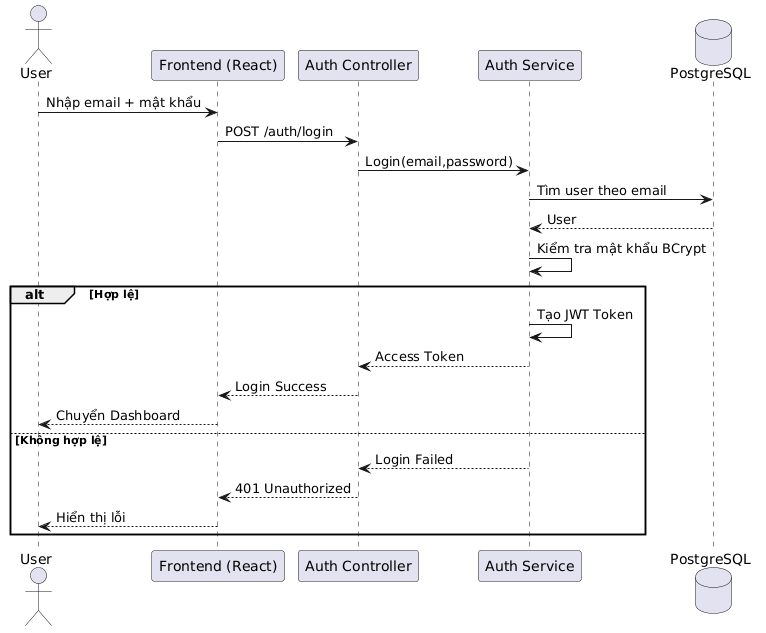
\includegraphics[width=\textwidth]{figures/sequence1.png}
\caption{Sequence Diagram chức năng đăng nhập hệ thống}
\label{fig:sequence_login}
\end{figure}

Mô hình tương tác thể hiện rõ lớp bảo mật tại tầng dịch vụ (\texttt{AuthService}). Tiến trình băm mật khẩu đối sánh được xử lý tuần tự trước khi tạo chuỗi mã hóa \texttt{AccessToken} để Frontend lưu trữ và điều hướng màn hình.

\subsection{Sequence Diagram chức năng đăng dự án}
Sơ đồ tuần tự thể hiện các bước nghiệp vụ tạo bài đăng công nghệ mới kết hợp lưu trữ tệp tin đính kèm.

\begin{figure}[H]
\centering
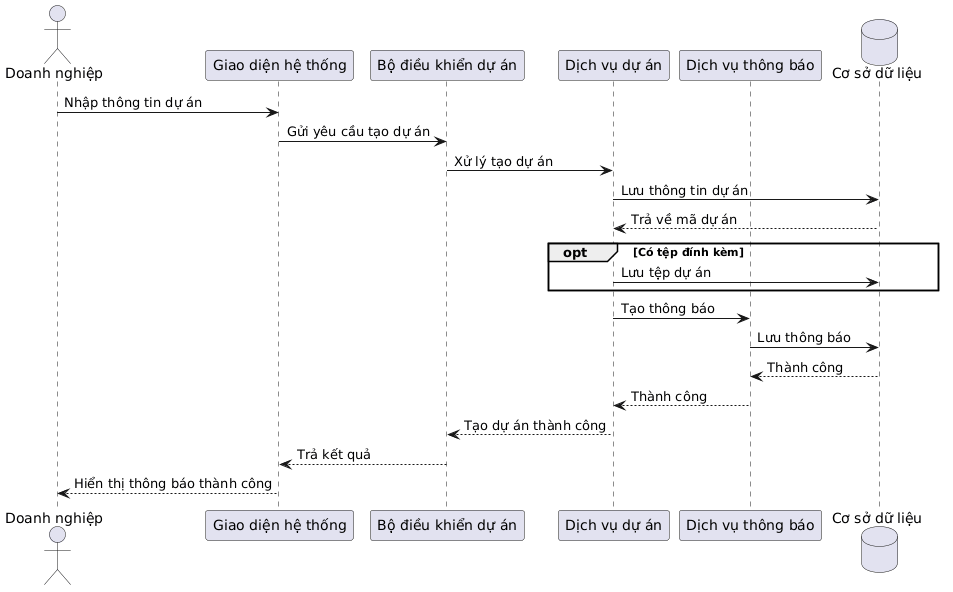
\includegraphics[width=\textwidth]{figures/sequence2.png}
\caption{Sequence Diagram chức năng đăng tải dự án}
\label{fig:sequence_create_project}
\end{figure}

Luồng xử lý bộc lộ tính kết hợp giữa lưu trữ dữ liệu cấu trúc (PostgreSQL) và xử lý tệp tin đa phương tiện. Khi \texttt{Project ID} được sinh ra, các tệp tài liệu đi kèm mới chính thức được ánh xạ và lưu vào hệ thống dữ liệu.

\subsection{Sequence Diagram chức năng gửi đề xuất}
Trình tự gọi hàm kiểm tra điều kiện ràng buộc nghiệp vụ khi chuyên gia gửi báo giá giải pháp.

\begin{figure}[H]
\centering
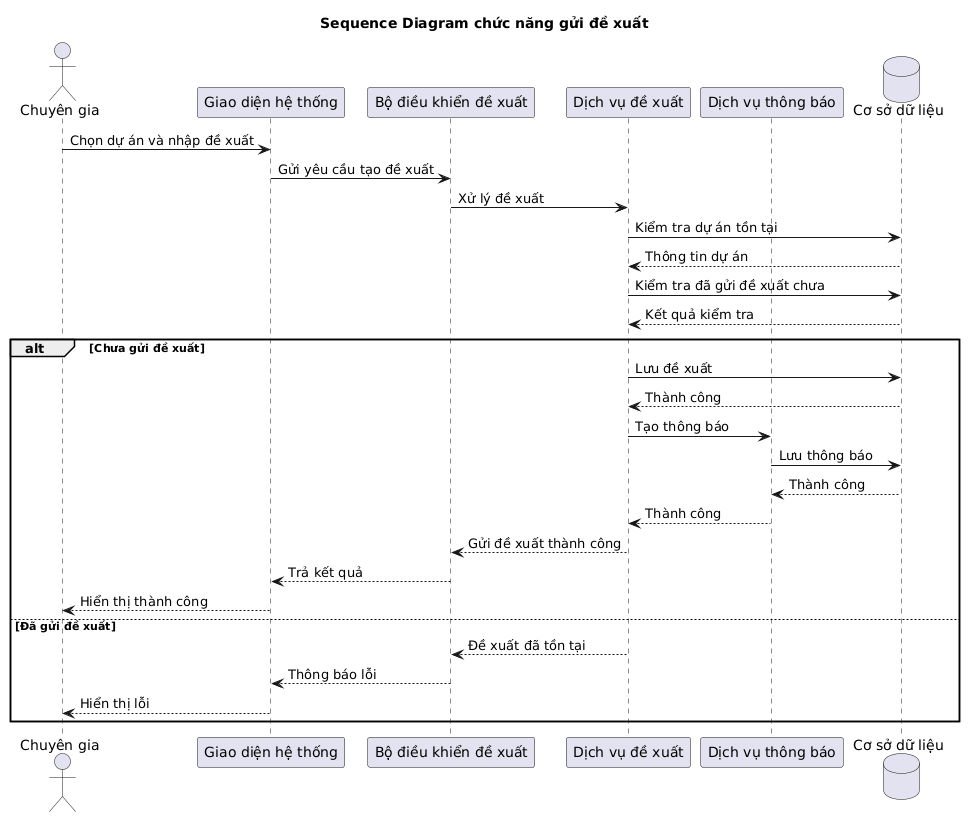
\includegraphics[width=\textwidth]{figures/sequence3.png}
\caption{Sequence Diagram chức năng chuyên gia gửi đề xuất}
\label{fig:sequence_send_proposal}
\end{figure}

Sơ đồ thể hiện kỹ thuật bẫy lỗi và chặn xử lý (Exception Handling) tại tầng nghiệp vụ. Hệ thống thực hiện các lệnh truy vấn kiểm tra điều kiện ràng buộc trước khi cho phép ghi dữ liệu đề xuất mới vào cơ sở dữ liệu.

\subsection{Sequence Diagram chức năng thuê chuyên gia}
Mô tả dòng chảy thông điệp phức tạp của tác vụ thay đổi trạng thái đồng loạt nhiều thực thể trong hệ thống.

\begin{figure}[H]
\centering
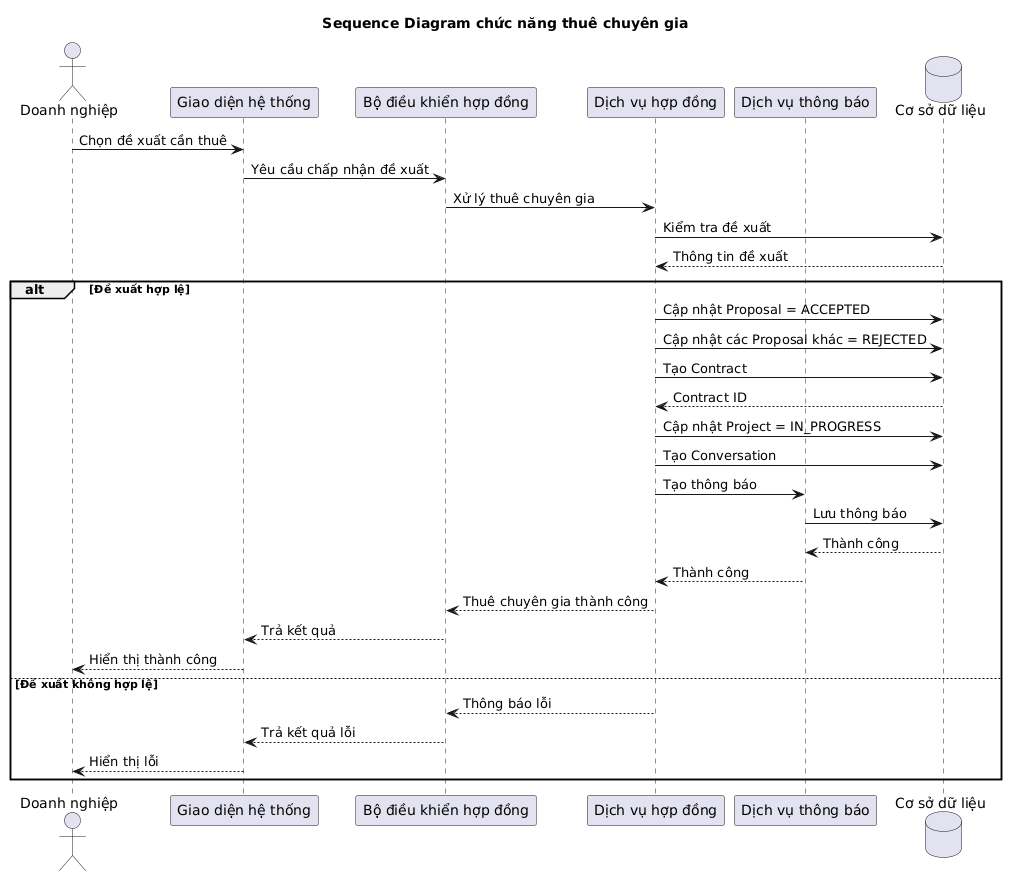
\includegraphics[width=\textwidth]{figures/sequence4.png}
\caption{Sequence Diagram chức năng phê duyệt và thuê chuyên gia}
\label{fig:sequence_hire_expert}
\end{figure}

Biểu đồ chỉ rõ tính liên kết chặt chẽ giữa các thành phần Controller, Service và Repository. Chuỗi hành động cập nhật trạng thái đề xuất, khởi tạo hợp đồng, đổi trạng thái dự án sang \texttt{IN\_PROGRESS} được thực thi tuần tự và đồng bộ.

\subsection{Sequence Diagram chức năng thanh toán}
Trình tự tương tác kết nối phân hệ tài chính nội bộ với cổng thanh toán điện tử trung gian bên thứ ba.

\begin{figure}[H]
\centering
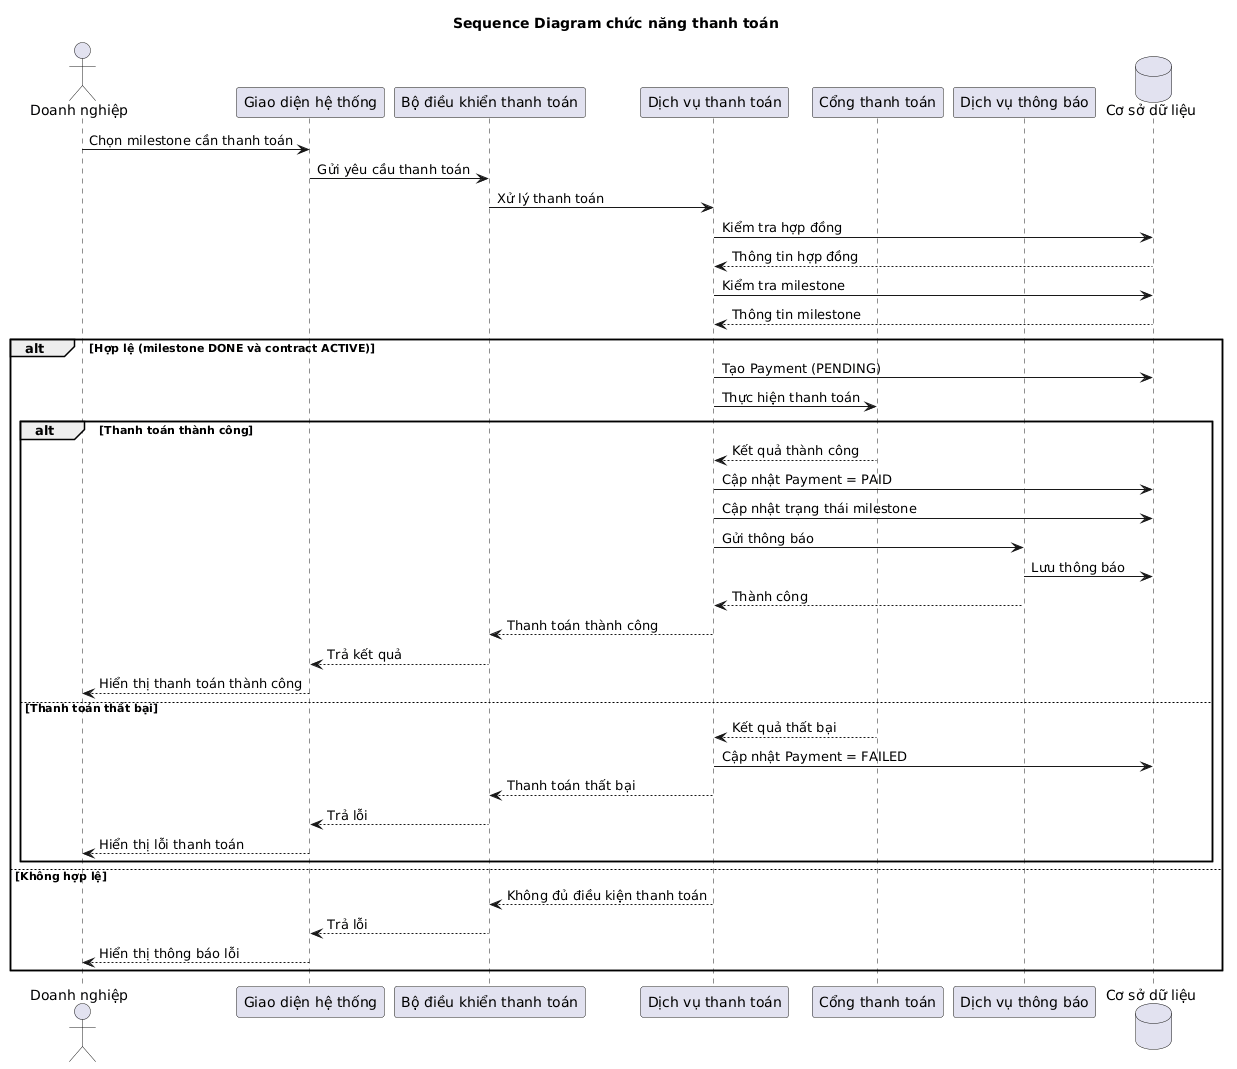
\includegraphics[width=\textwidth]{figures/sequence5.png}
\caption{Sequence Diagram chức năng thanh toán cột mốc công việc}
\label{fig:sequence_payment}
\end{figure}

Sơ đồ phân định rõ luồng xử lý bất đồng bộ khi đợi phản hồi kết quả giao dịch từ Cổng thanh toán ngoại vi (Payment Gateway). Bản ghi giao dịch được chuyển đổi trạng thái từ \texttt{PENDING} sang \texttt{PAID} hoặc \texttt{FAILED} dựa trên gói tin bảo mật trả về.

\subsection{Sequence Diagram chức năng đánh giá dự án}
Mô tả chi tiết luồng xử lý ghi nhận đánh giá và kích hoạt hàm cập nhật điểm tín nhiệm tự động.

\begin{figure}[H]
\centering
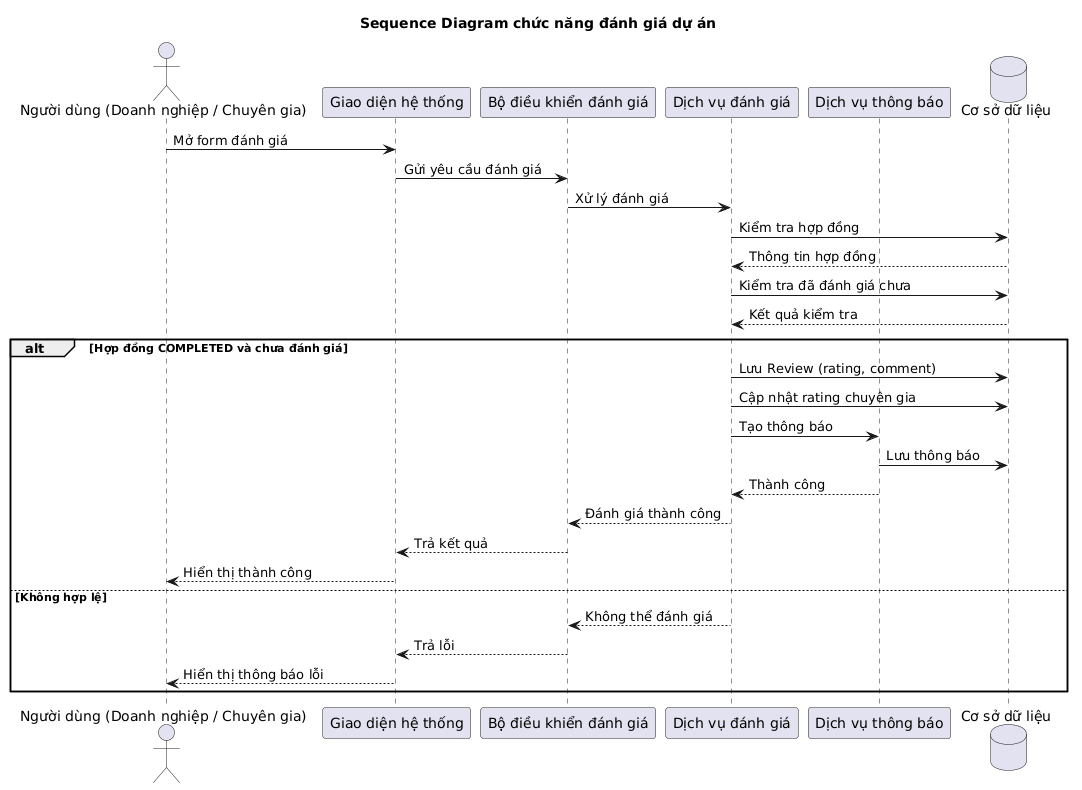
\includegraphics[width=\textwidth]{figures/sequence6.png}
\caption{Sequence Diagram chức năng đánh giá sau dự án}
\label{fig:sequence_review}
\end{figure}

Tiến trình tương tác tuần tự minh họa bước xử lý dữ liệu kép: vừa chèn bản ghi mới vào bảng \texttt{Reviews}, vừa gọi hàm tính toán cập nhật lại thuộc tính \texttt{rating} tích lũy của đối tượng nhận đánh giá tại bảng tương ứng.

\section{Biểu đồ lớp (Class Diagram)}

Class Diagram mô tả cấu trúc tĩnh, các thuộc tính định danh, các phương thức xử lý và mối liên kết logic giữa các thực thể mã nguồn của hệ thống AIConnect của hệ thống.

\begin{figure}[H]
\centering
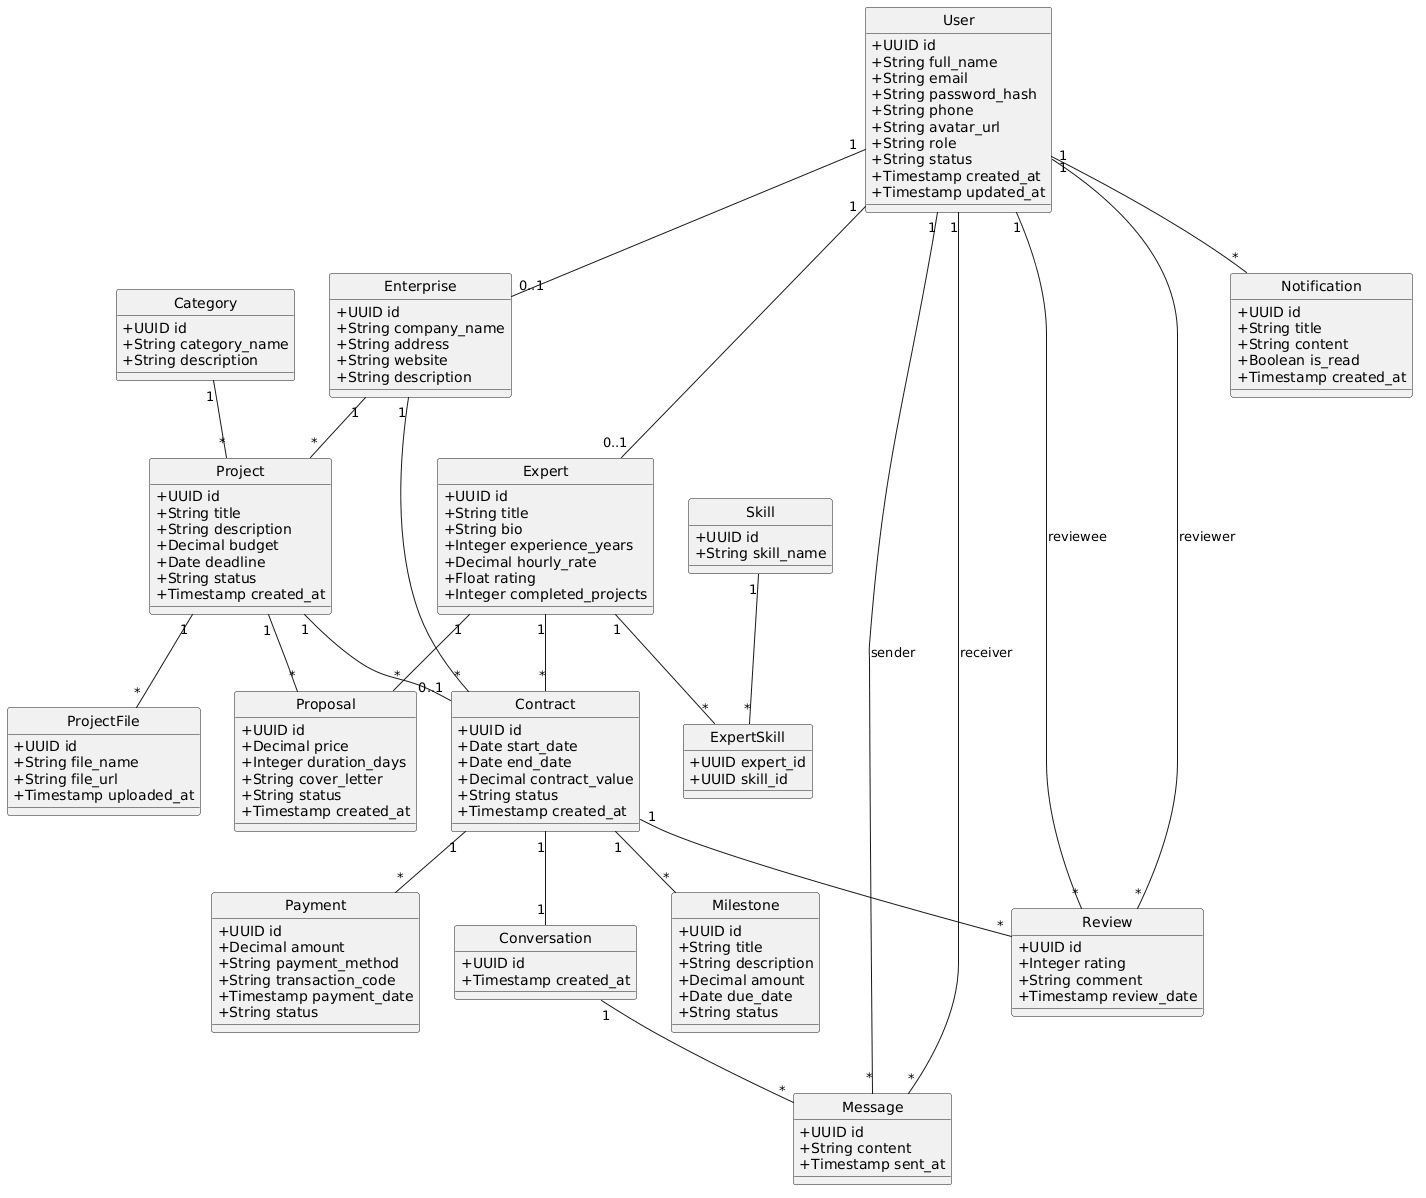
\includegraphics[width=\textwidth]{figures/Class.png}
\caption{Biểu đồ lớp (Class Diagram) hệ thống AIConnect}
\label{fig:class_diagram}
\end{figure}

Kiến trúc lớp thể hiện rõ mô hình thiết kế hướng đối tượng:
\begin{itemize}
    \item Lớp \texttt{User} đóng vai trò là lớp cơ sở chứa các thông tin định danh cốt lõi. \texttt{Enterprise} và \texttt{Expert} liên kết chuyên biệt hóa nhằm mở rộng các thuộc tính nghiệp vụ đặc thù.
    \item Lớp \texttt{Project} đóng vai trò trung tâm liên kết với lớp danh mục \texttt{Category} và quản lý danh sách các đề xuất ứng tuyển \texttt{Proposal}.
    \item Quy trình làm việc và tài chính được quản lý chặt chẽ thông qua mối quan hệ ràng buộc giữa \texttt{Contract}, \texttt{Milestone} và \texttt{Payment}.
\end{itemize}

\section{Biểu đồ ERD}

Entity Relationship Diagram (ERD) cụ thể hóa mô hình dữ liệu quan hệ, định hình cấu trúc các bảng và các ràng buộc toàn vẹn khóa chính (PK), khóa ngoại (FK) trong cơ sở dữ liệu PostgreSQL.

\begin{figure}[H]
\centering

\includegraphics[width=\textwidth]{figures/ERD.png}
\caption{Sơ đồ thực thể quan hệ (ERD) hệ thống AIConnect}
\label{fig:erd_diagram}
\end{figure}

Sơ đồ ERD ánh xạ toàn bộ các thực thể tĩnh từ mô hình lớp thành cấu trúc lưu trữ vật lý. Mối quan hệ nhiều - nhiều giữa chuyên gia và kỹ năng được giải quyết triệt để thông qua bảng trung gian \texttt{ExpertSkills}. Các thực thể động phát sinh trong quá trình vận hành như \texttt{Messages}, \texttt{Notifications} và \texttt{Reviews} đều được thiết lập khóa ngoại liên kết trực tiếp với các định danh người dùng và hợp đồng, đảm bảo tính tra cứu và toàn vẹn dữ liệu ở mức tối đa.

\section{Kết luận chương}

Chương này đã trình bày quá trình khảo sát và phân tích yêu cầu của hệ thống \textbf{AITasker – AI Marketplace Platform for AI Automation Services}. Thông qua việc phân tích bài toán thực tế, chương đã làm rõ bối cảnh, thực trạng, nhu cầu của người dùng cũng như các mục tiêu mà hệ thống cần đáp ứng.
Trên cơ sở đó, tài liệu đặc tả yêu cầu phần mềm (Software Requirement Specification -- SRS) đã được xây dựng, bao gồm việc xác định các tác nhân tham gia, các yêu cầu chức năng và phi chức năng của hệ thống. Đồng thời, các chức năng chính như quản lý người dùng, quản lý dự án AI, gửi báo giá, trao đổi giữa doanh nghiệp và chuyên gia, theo dõi tiến độ, đánh giá và quản trị hệ thống đã được phân tích một cách chi tiết.
Bên cạnh việc đặc tả yêu cầu, chương cũng xây dựng các mô hình UML gồm Use Case Diagram, Activity Diagram, Sequence Diagram, Class Diagram và Entity Relationship Diagram (ERD). Các mô hình này mô tả trực quan quy trình nghiệp vụ, luồng xử lý và mối quan hệ giữa các thành phần trong hệ thống, góp phần bảo đảm tính nhất quán trong quá trình phân tích và thiết kế.
Những kết quả đạt được trong chương là cơ sở quan trọng cho việc thiết kế kiến trúc hệ thống, cơ sở dữ liệu và triển khai các chức năng của nền tảng \textbf{AITasker} ở các chương tiếp theo. Đồng thời, các yêu cầu được xác định trong chương này cũng là căn cứ để kiểm thử và đánh giá mức độ hoàn thiện của hệ thống sau khi xây dựng.